% Supplementary material -- Explainable production-adjusted electrical-energy baselines for industrial feed pelleting
% Tables in tables/ are generated by build_tables.py from the archived aggregate results of the public repository.
\documentclass[11pt,a4paper]{article}
\usepackage[T1]{fontenc}\usepackage[utf8]{inputenc}
\usepackage{newtxtext,newtxmath}
\usepackage[margin=22mm]{geometry}
\usepackage{amsmath,booktabs,tabularx,array,graphicx,placeins,microtype,xcolor}
\usepackage[font=small,labelfont=bf]{caption}
\usepackage[hyphens]{url}
\usepackage[colorlinks=true,linkcolor=black,citecolor=black,urlcolor=blue!45!black]{hyperref}
\renewcommand{\thesection}{S\arabic{section}}
\renewcommand{\thetable}{S\arabic{table}}
\renewcommand{\thefigure}{S\arabic{figure}}
\newcommand{\ind}{\mathbf{1}}
\setlength{\parskip}{3pt}
\title{\vspace{-2em}\large Supplementary material to\\[4pt]\Large\bfseries Explainable production-adjusted electrical-energy baselines for industrial feed pelleting}
\author{\normalsize Vladimir Sousa Santos$^{a}$, Juan Jos\'e Cabello Eras$^{b}$,\\ \normalsize Eder El\'{\i}as Herrera Rodi\~no$^{c}$, Francisco Manuel Arrabal-Campos$^{d,*}$\\[4pt]
\footnotesize $^{a}$Department of Energy, Universidad de la Costa, Barranquilla, Colombia\\
\footnotesize $^{b}$Department of Mechanical Engineering, Faculty of Engineering, Universidad de C\'ordoba, Monter\'{\i}a, Colombia\\
\footnotesize $^{c}$Master's Programme in Mechanical Engineering, Universidad de C\'ordoba, Monter\'{\i}a, Colombia\\
\footnotesize $^{d}$Department of Engineering, Research Centre CIAIMBITAL, Escuela Superior de Ingenier\'{\i}a, University of Almer\'{\i}a, Spain\\
\footnotesize $^{*}$Corresponding author: fmarrabal@ual.es}
\date{}

\begin{document}
\maketitle

\section{Contents}
This document complements the main text with material that was not reproduced there: the complete source-variable dictionary and descriptive statistics of the industrial records (Section~\ref{sec:data}), the encoding and the full coefficient table of the frozen Ridge model (Section~\ref{sec:ridge}), the reference estimators and the development comparison at full precision (Section~\ref{sec:dev}), the block-bootstrap and multiplicity procedures (Section~\ref{sec:boot}), the calibration arithmetic of the residual intervals with line- and week-level diagnostics (Section~\ref{sec:intervals}), the protocol and stratified results of the matched temporal benchmark (Section~\ref{sec:temporal}), the CPU--GPU computational diagnostics (Section~\ref{sec:compute}) and the reproducibility and data-access arrangements (Section~\ref{sec:repro}). Every number is taken from the archived aggregate results distributed with the public repository; the tables were generated from those files by the script \texttt{build\_tables.py} included with this document.

\section{Source data}\label{sec:data}
Table~\ref{tab:s_variables} lists the 32 fields of the plant workbook, the name used in the analytical table, the role each field plays in the study and whether its value can be assumed to exist at the prediction origin. Only ten fields enter the baseline: dosed mass, dosing-batch count, pelleting line, product subfamily, presentation and bag/bulk category, plus the origin hour and weekday derived from the earliest recorded stage start. Energy, duration, steam, temperature and current summaries of the current record are not used, because the workbook does not establish when they become available. The timestamps of milling and mixing define the analytical origin together with the pelleting start, whereas the completion timestamps are used only to decide which historical outcomes are admissible for the temporal analyses.

The analytical table was reconciled cell by cell with the workbook: 32 fields $\times$ 2,745 records = 87,840 comparisons, all within the documented numerical and whitespace tolerances (last column of Table~\ref{tab:s_variables}). The three records with zero pelleting energy were kept in the audit and excluded from every supervised target. Missing values occur only in auxiliary operational summaries and in two stage timestamps; the fifteen auxiliary values that had been imputed during preparation belong to fields that are not model inputs.

\begin{table}[!htbp]\centering\scriptsize
\caption{The 32 source fields of the plant workbook, their analytical names, role in the study, availability at the prediction origin, number of missing values in the source and cells matched in the fidelity reconciliation.}\label{tab:s_variables}
\begin{tabularx}{\linewidth}{@{}>{\raggedright\arraybackslash}p{.16\linewidth}>{\raggedright\arraybackslash}p{.23\linewidth}>{\raggedright\arraybackslash}p{.15\linewidth}>{\raggedright\arraybackslash}Xrr@{}}\toprule
Source field & Analytical name & Role & Availability at origin & Missing & Matched \\\midrule
\texttt{DES\_\allowbreak{}PRODUCTO\_\allowbreak{}TIPO} & \texttt{salida\_\allowbreak{}programada} & model input & not verified before origin & 0 & 2,745/2,745 \\
\texttt{N\_\allowbreak{}BACHES\_\allowbreak{}DOS} & \texttt{baches\_\allowbreak{}dosificacion} & model input & not verified before origin & 0 & 2,745/2,745 \\
\texttt{PESO DOS (kg)} & \texttt{masa\_\allowbreak{}dosificada\_\allowbreak{}kg} & model input & not verified before origin & 0 & 2,745/2,745 \\
\texttt{PELLT} & \texttt{linea} & model input & not verified before origin & 0 & 2,745/2,745 \\
\texttt{CANTIDAD\_\allowbreak{}BACHES\_\allowbreak{}PEL} & \texttt{baches\_\allowbreak{}peletizado} & op. summary (unused) & after origin / undocumented & 0 & 2,745/2,745 \\
\texttt{CANT PELETIZADA} & \texttt{produccion\_\allowbreak{}t\_\allowbreak{}asumida} & op. summary (unused) & after origin / undocumented & 0 & 2,745/2,745 \\
\texttt{KWH PELET} & \texttt{energia\_\allowbreak{}peletizado\_\allowbreak{}kWh} & target & after origin & 0 & 2,745/2,745 \\
\texttt{PRESION VAPOR (psi)} & \texttt{presion\_\allowbreak{}vapor\_\allowbreak{}psig} & op. summary (unused) & after origin / undocumented & 0 & 2,745/2,745 \\
\texttt{VAPOR (Lb)} & \texttt{masa\_\allowbreak{}vapor\_\allowbreak{}lb} & op. summary (unused) & after origin / undocumented & 0 & 2,745/2,745 \\
\texttt{TEMP\_\allowbreak{}ACONDICIONADOR} & \texttt{temperatura\_\allowbreak{}acond\_\allowbreak{}C} & op. summary (unused) & after origin / undocumented & 7 & 2,745/2,745 \\
\texttt{AMPERAJE\_\allowbreak{}PEL} & \texttt{corriente\_\allowbreak{}peletizado\_\allowbreak{}A} & op. summary (unused) & after origin / undocumented & 0 & 2,745/2,745 \\
\texttt{FEC\_\allowbreak{}INI\_\allowbreak{}PEL\_\allowbreak{}TS} & \texttt{inicio\_\allowbreak{}peletizado} & chronology: origin & event observation & 2 & 2,745/2,745 \\
\texttt{FEC\_\allowbreak{}FIN\_\allowbreak{}PEL\_\allowbreak{}TS} & \texttt{fin\_\allowbreak{}peletizado} & chronology: labels & after origin & 2 & 2,745/2,745 \\
\texttt{N\_\allowbreak{}BACHES\_\allowbreak{}MOL} & \texttt{baches\_\allowbreak{}molienda} & op. summary (unused) & after origin / undocumented & 2 & 2,745/2,745 \\
\texttt{FEC\_\allowbreak{}INI\_\allowbreak{}MOL} & \texttt{inicio\_\allowbreak{}molienda} & chronology: origin & event observation & 2 & 2,745/2,745 \\
\texttt{FEC\_\allowbreak{}FIN\_\allowbreak{}MOL} & \texttt{fin\_\allowbreak{}molienda} & chronology: labels & after origin & 2 & 2,745/2,745 \\
\texttt{KWH MOL} & \texttt{energia\_\allowbreak{}molienda\_\allowbreak{}kWh} & op. summary (unused) & after origin / undocumented & 0 & 2,745/2,745 \\
\texttt{TEMP\_\allowbreak{}DEVANADO} & \texttt{temperatura\_\allowbreak{}devanado\_\allowbreak{}C} & op. summary (unused) & after origin / undocumented & 5 & 2,745/2,745 \\
\texttt{TEMP\_\allowbreak{}ROD\_\allowbreak{}DELANTERO} & \texttt{temperatura\_\allowbreak{}rod\_\allowbreak{}del\_\allowbreak{}C} & op. summary (unused) & after origin / undocumented & 5 & 2,745/2,745 \\
\texttt{TEMP\_\allowbreak{}ROD\_\allowbreak{}TRASERO} & \texttt{temperatura\_\allowbreak{}rod\_\allowbreak{}tras\_\allowbreak{}C} & op. summary (unused) & after origin / undocumented & 5 & 2,745/2,745 \\
\texttt{AMPERAJE\_\allowbreak{}MOL} & \texttt{corriente\_\allowbreak{}molienda\_\allowbreak{}A} & op. summary (unused) & after origin / undocumented & 0 & 2,745/2,745 \\
\texttt{N\_\allowbreak{}BACHES\_\allowbreak{}MEZ} & \texttt{baches\_\allowbreak{}mezclado} & op. summary (unused) & after origin / undocumented & 2 & 2,745/2,745 \\
\texttt{FEC\_\allowbreak{}INI\_\allowbreak{}MEZ} & \texttt{inicio\_\allowbreak{}mezclado} & chronology: origin & event observation & 2 & 2,745/2,745 \\
\texttt{FEC\_\allowbreak{}FIN\_\allowbreak{}MEZ} & \texttt{fin\_\allowbreak{}mezclado} & chronology: labels & after origin & 2 & 2,745/2,745 \\
\texttt{KWH MEZ} & \texttt{energia\_\allowbreak{}mezclado\_\allowbreak{}kWh} & op. summary (unused) & after origin / undocumented & 0 & 2,745/2,745 \\
\texttt{AMPERAJE\_\allowbreak{}MEZ} & \texttt{corriente\_\allowbreak{}mezclado\_\allowbreak{}A} & op. summary (unused) & after origin / undocumented & 0 & 2,745/2,745 \\
\texttt{UNIDADINVENTARIO} & \texttt{unidad\_\allowbreak{}inventario} & context (unused) & not verified before origin & 0 & 2,745/2,745 \\
\texttt{AGRUPACION\_\allowbreak{}INVENTARIO} & \texttt{grupo\_\allowbreak{}inventario} & context (unused) & not verified before origin & 0 & 2,745/2,745 \\
\texttt{LINEA} & \texttt{familia} & context (unused) & not verified before origin & 0 & 2,745/2,745 \\
\texttt{SUBLINEA} & \texttt{subfamilia} & model input & not verified before origin & 0 & 2,745/2,745 \\
\texttt{PRESENTACION} & \texttt{forma} & model input & not verified before origin & 0 & 2,745/2,745 \\
\texttt{EMPAQUE} & \texttt{empaque\_\allowbreak{}final} & context (unused) & not verified before origin & 0 & 2,745/2,745 \\
\bottomrule
\end{tabularx}
\par\vspace{3pt}\footnotesize Original Spanish field names are retained for traceability. Model inputs are admitted for the retrospective baseline; prospective use would require a plan version and a timestamp before the origin. The fidelity reconciliation compared every cell of the analytical table with the workbook under the documented tolerances: 32 fields $\times$ 2,745 records = 87,840 comparisons, all matched.
\end{table}

\begin{table}[!htbp]\centering\small
\caption{Descriptive statistics of the numerical variables over all 2,745 source records (including the three zero-energy records). Pearson correlation between dosed mass and dosing-batch count: 0.979.}\label{tab:s_numeric}
\begin{tabular}{@{}lrrrrrrrr@{}}\toprule
Variable & $n$ & Mean & SD & Min & Q1 & Median & Q3 & Max \\\midrule
Dosed mass (t) & 2,745 & 13.92 & 5.73 & 2.69 & 10.79 & 14.98 & 18.03 & 36.78 \\
Dosing batches & 2,745 & 3.95 & 1.54 & 1.00 & 3.00 & 5.00 & 5.00 & 10.00 \\
Pelleting electricity (kWh) & 2,745 & 258.16 & 124.07 & 0.00 & 179.10 & 251.10 & 320.40 & 1075.50 \\
\bottomrule
\end{tabular}
\end{table}

\begin{table}[!htbp]\centering\footnotesize
\caption{Record counts of every categorical level in the 2,745 source records. Family (\texttt{LINEA}) is context only; line, subfamily, presentation and bag/bulk are model inputs.}\label{tab:s_categories}
\begin{tabular}{@{}llr@{}}\toprule
Field & Level & Records \\\midrule
Pelleting line & \texttt{Pellet 2} & 1,148 \\
Pelleting line & \texttt{Pellet 3} & 867 \\
Pelleting line & \texttt{Pellet 1} & 730 \\
Product family & \texttt{LINEA PORCICULTURA} & 1,242 \\
Product family & \texttt{LINEA AVICULTURA} & 1,123 \\
Product family & \texttt{LINEA GANADERIA} & 299 \\
Product family & \texttt{LINEA EQUINOS} & 55 \\
Product family & \texttt{LINEA OTROS} & 26 \\
Product subfamily & \texttt{SUBLINEA AVICULTURA ENGORDE} & 797 \\
Product subfamily & \texttt{SUBLINEA PORCICULTURA CEBA} & 783 \\
Product subfamily & \texttt{SUBLINEA PORCICULTURA CRIA} & 359 \\
Product subfamily & \texttt{SUBLINEA AVICULTURA POSTURA} & 326 \\
Product subfamily & \texttt{SUBLINEA GANADERIA LECHE} & 238 \\
Product subfamily & \texttt{SUBLINEA PORCICULTURA PREINICIADORES} & 100 \\
Product subfamily & \texttt{SUBLINEA GANADERIA CARNE} & 61 \\
Product subfamily & \texttt{SUBLINEA EQUINOS} & 55 \\
Product subfamily & \texttt{SUBLINEA OTROS CONEJOS} & 26 \\
Presentation & \texttt{PELETIZADO} & 2,065 \\
Presentation & \texttt{CROMBELIZADO} & 680 \\
Bag/bulk & \texttt{ENSAQUE} & 2,420 \\
Bag/bulk & \texttt{GRANEL} & 325 \\
\bottomrule
\end{tabular}
\end{table}


Table~\ref{tab:s_temporal} summarizes the temporal structure of the records per line and Table~\ref{tab:s_flow} the chronological partitions. Development and calibration eligibility require a positive recorded outcome, a valid duration, complete required inputs and completion before the next partition boundary; this removes 14 development and 11 calibration candidates, whereas all 798 test candidates are retained.

\begin{table}[!htbp]\centering\small
\caption{Temporal structure of the records by pelleting line: records, positive targets, within-line overlaps with the previous interval, operations longer than 24 h, median minutes between consecutive starts and median recorded pelleting duration.}\label{tab:s_temporal}
\begin{tabular}{@{}lrrrrrr@{}}\toprule
Line & Records & Positive targets & Overlaps & $>$24 h & Median gap (min) & Median duration (min) \\\midrule
Pellet 1 & 730 & 729 & 75 & 3 & 152.1 & 145.1 \\
Pellet 2 & 1,148 & 1,146 & 131 & 6 & 93.0 & 96.0 \\
Pellet 3 & 867 & 867 & 145 & 8 & 124.1 & 123.1 \\
\bottomrule
\end{tabular}
\end{table}

\begin{table}[!htbp]\centering\small
\caption{Chronological partitions: candidate records, records retained after the eligibility rules, exclusions and the range of analytical origins (earliest recorded stage start).}\label{tab:s_flow}
\begin{tabular}{@{}lrrrll@{}}\toprule
Partition & Candidates & Retained & Excluded & First origin & Last origin \\\midrule
Development & 1,556 & 1,542 & 14 & 2025-01-02 10:12 & 2025-02-21 22:34 \\
Calibration & 391 & 380 & 11 & 2025-02-22 00:06 & 2025-03-05 23:12 \\
Test & 798 & 798 & 0 & 2025-03-06 00:00 & 2025-04-01 17:28 \\
\bottomrule
\end{tabular}
\end{table}

\FloatBarrier

\section{Encoding and the frozen Ridge model}\label{sec:ridge}
Each numerical coordinate $x$ is standardized with the training mean $\bar x_{\mathrm{train}}$ and standard deviation $s_{\mathrm{train}}$ of the corresponding training block, $z=(x-\bar x_{\mathrm{train}})/s_{\mathrm{train}}$, and each categorical field is expanded into one indicator per level present in the training vocabulary. For the frozen model fitted on the 1,542 eligible development records this yields $6+3+9+2+2=22$ design columns: six numerical coordinates, three pelleting lines, nine product subfamilies, two presentations and two bag/bulk levels. A level absent from the training vocabulary activates no indicator of its field; no such level occurred in the calibration or test periods.

The model minimizes the penalized squared error of the main text with an unpenalized intercept and penalty 10 on the coefficient vector (scikit-learn \texttt{Ridge(alpha=10)} on the transformed design). Table~\ref{tab:s_coefficients} gives all 22 coefficients and Table~\ref{tab:s_effects} converts the numerical coefficients back to original units, $\beta_{\mathrm{unit}}=\beta_{\mathrm{SD}}/s_{\mathrm{train}}$: 73.9003~kWh per training standard deviation of dosed mass (5.5556~t) is 13.3018~kWh per tonne, and 14.2309~kWh per standard deviation of batch count (1.4943 batches) is 9.5233~kWh per batch. The intercept, 288.09~kWh, is the value of the untruncated predictor at standardized means with all indicators at zero and is not a physical standby consumption. The grouped decomposition $f_i=\widehat b+\sum_g C_{ig}$ was recomputed for the 798 archived test estimates with a maximum absolute discrepancy of $1.14\times10^{-13}$~kWh; no estimate required clipping at zero.

\begin{table}[!htbp]\centering\footnotesize
\caption{All 22 coefficients of the frozen Ridge model (penalty 10, fitted on 1,542 development records). Intercept: 288.09 kWh. Numerical coefficients are per training standard deviation; one-hot coefficients are per indicator.}\label{tab:s_coefficients}
\begin{tabular}{@{}llr@{}}\toprule
Encoded variable & Type & Coefficient (kWh) \\\midrule
Dosed mass & numerical (per training SD) & 73.9003 \\
Dosing batches & numerical (per training SD) & 14.2309 \\
Origin hour, sine & numerical (per training SD) & 0.1912 \\
Origin hour, cosine & numerical (per training SD) & $-0.0496$ \\
Weekday, sine & numerical (per training SD) & $-1.8094$ \\
Weekday, cosine & numerical (per training SD) & $-1.4544$ \\
\texttt{Pellet 1} & pelleting line (one-hot) & $-0.7987$ \\
\texttt{Pellet 2} & pelleting line (one-hot) & 0.1181 \\
\texttt{Pellet 3} & pelleting line (one-hot) & 0.6806 \\
\texttt{SUBLINEA AVICULTURA ENGORDE} & product subfamily (one-hot) & $-10.9350$ \\
\texttt{SUBLINEA AVICULTURA POSTURA} & product subfamily (one-hot) & $-27.4928$ \\
\texttt{SUBLINEA EQUINOS} & product subfamily (one-hot) & 5.2334 \\
\texttt{SUBLINEA GANADERIA CARNE} & product subfamily (one-hot) & $-20.7153$ \\
\texttt{SUBLINEA GANADERIA LECHE} & product subfamily (one-hot) & 11.0388 \\
\texttt{SUBLINEA OTROS CONEJOS} & product subfamily (one-hot) & 4.9565 \\
\texttt{SUBLINEA PORCICULTURA CEBA} & product subfamily (one-hot) & $-52.8982$ \\
\texttt{SUBLINEA PORCICULTURA CRIA} & product subfamily (one-hot) & 23.0575 \\
\texttt{SUBLINEA PORCICULTURA PREINICIADORES} & product subfamily (one-hot) & 67.7552 \\
\texttt{CROMBELIZADO} & presentation (one-hot) & 54.3247 \\
\texttt{PELETIZADO} & presentation (one-hot) & $-54.3247$ \\
\texttt{programada\_ENSAQUE} & bag/bulk (one-hot) & 15.5600 \\
\texttt{programada\_GRANEL} & bag/bulk (one-hot) & $-15.5600$ \\
\bottomrule
\end{tabular}
\par\vspace{3pt}\footnotesize With an unpenalized intercept and complete one-hot sets, the penalized solution centres each categorical set, which is why the two-level fields (presentation, bag/bulk) carry opposite coefficients of equal magnitude.
\end{table}

\begin{table}[!htbp]\centering\small
\caption{Conversion of the numerical Ridge coefficients from standardized to original units: $\beta_{\mathrm{unit}}=\beta_{\mathrm{SD}}/s_{\mathrm{train}}$, with the training mean and standard deviation used for standardization.}\label{tab:s_effects}
\begin{tabular}{@{}lrrrr@{}}\toprule
Variable & Coef. per training SD (kWh) & Training mean & Training SD & Coef. per original unit (kWh) \\\midrule
Dosed mass (t) & 73.9003 & 14.1169 & 5.5556 & 13.3018 \\
Dosing batches & 14.2309 & 4.0208 & 1.4943 & 9.5233 \\
Origin hour, sine & 0.1912 & $-0.0114$ & 0.7092 & 0.2696 \\
Origin hour, cosine & $-0.0496$ & 0.0391 & 0.7038 & $-0.0704$ \\
Weekday, sine & $-1.8094$ & 0.1019 & 0.6747 & $-2.6816$ \\
Weekday, cosine & $-1.4544$ & $-0.0913$ & 0.7252 & $-2.0053$ \\
\bottomrule
\end{tabular}
\end{table}

\FloatBarrier

\section{Reference estimators and development comparison}\label{sec:dev}
Three operational references were evaluated alongside the fitted models. The line-specific SEC reference multiplies the dosed mass by the ratio of total training energy to total training mass of the same line. The recent-SEC reference uses the median of the last five completed same-line energy-to-mass ratios and is the only reference whose information is updated as outcomes become available during a validation week. The line-specific median reference predicts the training median energy of the line irrespective of mass. Table~\ref{tab:s_development} reports the development comparison on the 800 common targets at full archived precision, together with the three post-hoc extensions of the Ridge model: H1 adds a mass$\times$line interaction, H2 a mass$\times$subfamily interaction and H3 a shrunk correction from up to 20 recent same-line residuals of the frozen model ($\delta_i=\tfrac{n_i}{n_i+10}\bar e_i$ for $n_i\ge5$, otherwise zero). Table~\ref{tab:s_contrasts} gives their paired contrasts and Figure~\ref{fig:s_dev} the corresponding figure.

\begin{table}[!htbp]\centering\small
\caption{Development performance on the same 800 chronological targets at full archived precision: the seven original methods and the three post-hoc extensions of the Ridge model. MAE, RMSE and bias in kWh per record.}\label{tab:s_development}
\begin{tabular}{@{}lrrrrr@{}}\toprule
Method & $n$ & MAE & RMSE & Bias & WAPE (\%) \\\midrule
Ridge & 800 & 51.4810 & 72.3097 & $-3.1361$ & 19.88 \\
Gradient boosting & 800 & 51.4969 & 73.4650 & $-5.7223$ & 19.88 \\
ExtraTrees & 800 & 52.3138 & 75.3733 & $-4.8856$ & 20.20 \\
MLP, three-seed mean & 800 & 56.6418 & 81.3564 & $-1.4663$ & 21.87 \\
Line-specific SEC & 800 & 59.6911 & 83.9218 & $-6.5940$ & 23.05 \\
Recent SEC, last five records & 800 & 73.5101 & 109.5456 & 4.2886 & 28.38 \\
Line-specific median & 800 & 82.6053 & 112.7830 & $-14.0866$ & 31.89 \\
H1: mass by pelleting line & 800 & 51.2644 & 72.1061 & $-3.1829$ & 19.79 \\
H2: mass by product subfamily & 800 & 50.0392 & 71.2040 & $-3.8264$ & 19.32 \\
H3: recent-residual correction & 800 & 49.7687 & 70.6723 & $-0.6798$ & 19.21 \\
\bottomrule
\end{tabular}
\end{table}

\begin{table}[!htbp]\centering\small\setlength{\tabcolsep}{4pt}
\caption{Paired MAE reductions of the exploratory extensions relative to the frozen Ridge specification on the 800 development targets: block-bootstrap percentile intervals (5,000 replicates, blocks of three observed origin dates) at the marginal 95\% level and at the Bonferroni-adjusted 98.33\% level for the three comparisons.}\label{tab:s_contrasts}
\begin{tabular}{@{}lrrll@{}}\toprule
Extension & Reduction (kWh) & Reduction (\%) & 95\% interval (kWh) & 98.33\% interval (kWh) \\\midrule
H1: mass by pelleting line & 0.217 & 0.42 & [$-0.034$, 0.500] & [$-0.082$, 0.581] \\
H2: mass by product subfamily & 1.442 & 2.80 & [0.701, 2.296] & [0.552, 2.481] \\
H3: recent-residual correction & 1.712 & 3.33 & [0.486, 2.913] & [0.236, 3.156] \\
\bottomrule
\end{tabular}
\end{table}


\begin{figure}[!htbp]\centering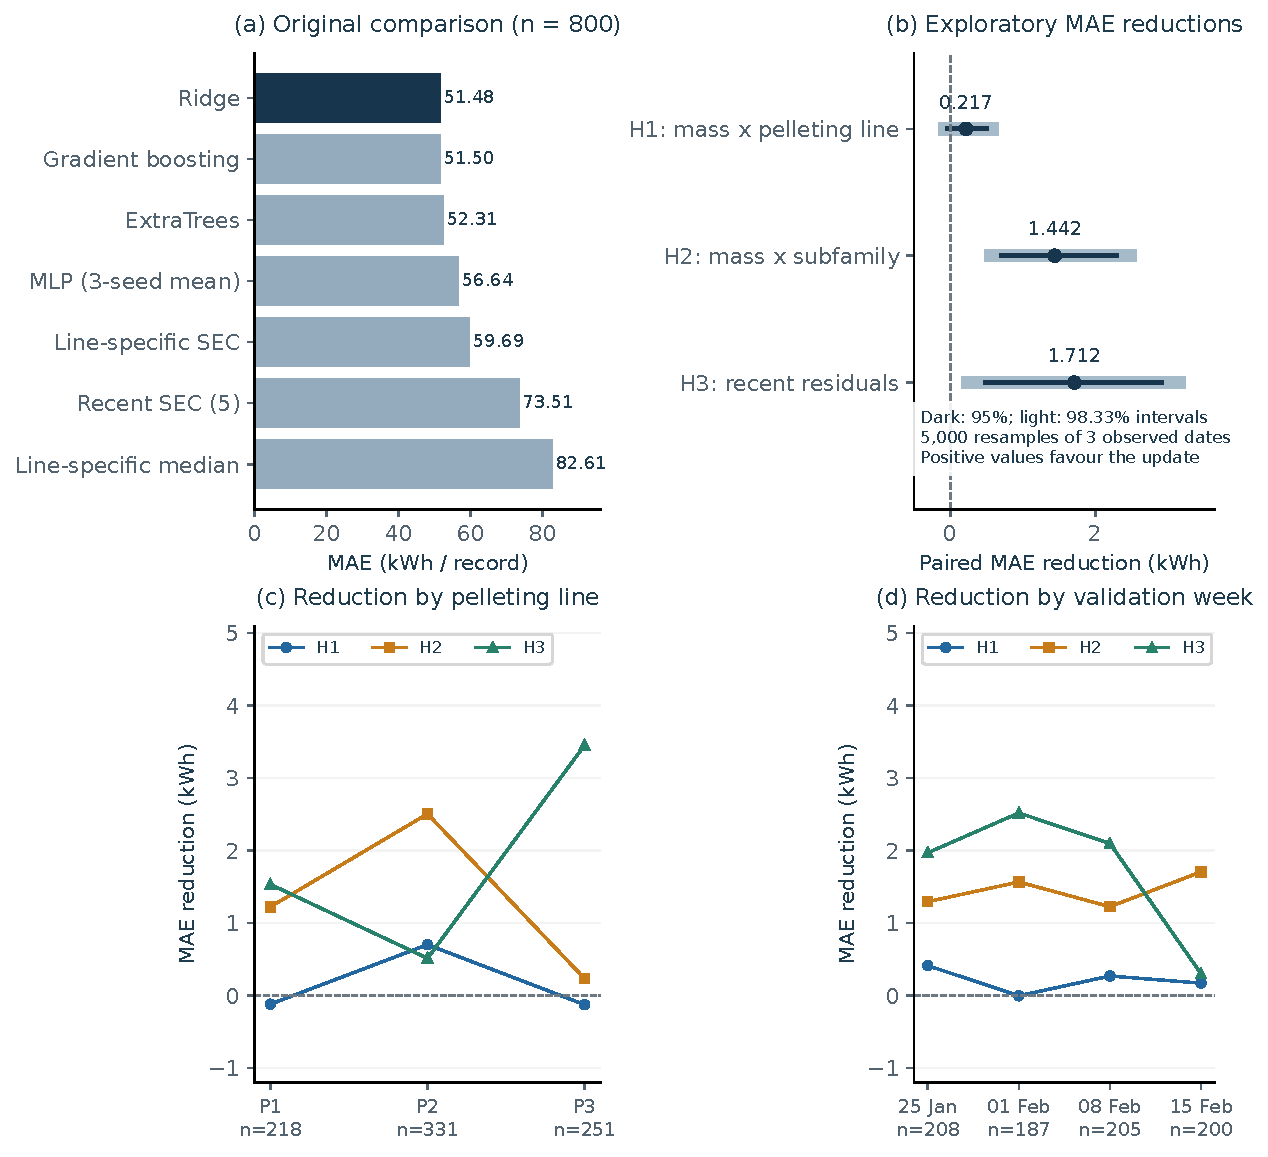
\includegraphics[width=\linewidth]{figures/03_development_and_hypotheses.pdf}
\caption{Development results and exploratory extensions. (a) MAE of the seven original methods on the 800 common development records. (b) Paired MAE reductions relative to Ridge for line-dependent mass effects (H1), product-dependent mass effects (H2) and recent-residual correction (H3), with 95\% and multiplicity-adjusted 98.33\% intervals. (c,d) Reductions by pelleting line and by validation week; positive values favour the extension.}\label{fig:s_dev}\end{figure}
\FloatBarrier

\section{Block bootstrap and multiplicity}\label{sec:boot}
All paired comparisons use a circular block bootstrap over observed origin dates. Let $n_d$ be the number of dates with at least one target (27 in the test period, 28 in the development weeks, 21 in the matched temporal benchmark). Each replicate draws $\lceil n_d/3\rceil$ random starting dates, takes each start and the two following dates modulo $n_d$, truncates the sequence to $n_d$ dates and keeps every record of every selected date, so that all lines recorded on the same date remain together. The statistic (difference of mean absolute errors, or coverage) is recomputed from the resampled records, and the percentile interval is read from the replicate distribution. The number of replicates is 3,000 for the primary test comparison (random seed 20260920) and 5,000 for the exploratory extensions (seed 20260921) and the temporal benchmark (seed 20260922). On the test period this gives a paired MAE reduction of Ridge over line-specific SEC of 8.838~kWh with 95\% interval [6.076, 11.503]~kWh (14.42\%), and 95\% intervals of [81.86, 90.24]\% and [90.53, 95.87]\% for the empirical coverage of the fixed 90\% and 95\% intervals.

Families of contrasts use approximate Bonferroni adjustment of the percentile level: $1-0.05/3=0.9833$ for the three extensions and $1-0.05/7=0.9929$ for the seven temporal contrasts. The adjustment covers the contrasts explicitly stated within each family and not the earlier exploratory choices that motivated them.

\section{Residual intervals}\label{sec:intervals}
The frozen model's absolute calibration errors $r_j=|y_j-\widehat y_j|$ on the 380 calibration records are sorted, and the half-width at miscoverage $\alpha$ is the order statistic of rank $\lceil(n_{\mathrm{cal}}+1)(1-\alpha)\rceil$: rank $\lceil381\times0.90\rceil=343$ gives $q_{0.10}=93.0132$~kWh and rank $\lceil381\times0.95\rceil=362$ gives $q_{0.05}=132.9576$~kWh. The interval of record $i$ is $[\max(0,\widehat y_i-q_\alpha),\ \widehat y_i+q_\alpha]$.

For the worked example of the main text (source row 2080, Pellet~2, 18.002~t in five dosing batches, origin 10 March 2025 08:31), the archived estimate is 255.8964~kWh, the 90\% interval [162.8833, 348.9096]~kWh and the 95\% interval [122.9389, 388.8540]~kWh. The recorded energy, 267.3~kWh, gives a signed excess of 11.4036~kWh, both flags are zero, and the interval score at the 95\% level equals the width, 265.915~kWh, because no penalty term applies. Over the 798 test records the fixed 95\% intervals missed 54 outcomes (45 above the upper limit, 9 below the lower limit), i.e.\ 6.77 flagged records per 100 operations; the fixed 90\% intervals missed 112 (88 above, 24 below).

The rolling policy keeps the point estimates fixed and recomputes the half-widths, with the same rank rule, from the 200 most recent available absolute residuals (rank 181 of 200 at the 90\% level and 191 at the 95\% level), ordered by recorded pelleting completion and then by source row; the pool starts with the calibration residuals and admits a test residual only after the completion of its operation precedes the origin of the target being evaluated (159,600 donor relationships checked). Tables~\ref{tab:s_intervals_line} and \ref{tab:s_intervals_week} give coverage, width, interval score and exceedance counts by line and by week for both policies, and Figure~\ref{fig:s_unc} shows the trade-off.

\begin{table}[!htbp]\centering\footnotesize
\caption{Residual intervals by pelleting line on the 798 test records: empirical coverage, mean width, interval score and the number of records above (high) and below (low) the interval, for the fixed calibration and the post-hoc rolling update.}\label{tab:s_intervals_line}
\begin{tabular}{@{}lllrrrrrr@{}}\toprule
Policy & Nominal & Line & $n$ & Coverage (\%) & Width (kWh) & Score (kWh) & High & Low \\\midrule
Fixed & 90\% & Pellet 1 & 200 & 81.00 & 182.96 & 526.08 & 37 & 1 \\
Fixed & 90\% & Pellet 2 & 333 & 91.59 & 182.48 & 279.18 & 22 & 6 \\
Fixed & 90\% & Pellet 3 & 265 & 82.64 & 185.59 & 401.84 & 29 & 17 \\
Fixed & 95\% & Pellet 1 & 200 & 90.00 & 256.09 & 719.79 & 20 & 0 \\
Fixed & 95\% & Pellet 2 & 333 & 96.40 & 256.38 & 359.20 & 9 & 3 \\
Fixed & 95\% & Pellet 3 & 265 & 91.70 & 264.03 & 503.93 & 16 & 6 \\
Rolling, 200 residuals & 90\% & Pellet 1 & 200 & 86.00 & 215.78 & 493.40 & 27 & 1 \\
Rolling, 200 residuals & 90\% & Pellet 2 & 333 & 94.29 & 218.61 & 290.20 & 13 & 6 \\
Rolling, 200 residuals & 90\% & Pellet 3 & 265 & 86.04 & 224.15 & 399.77 & 26 & 11 \\
Rolling, 200 residuals & 95\% & Pellet 1 & 200 & 92.00 & 298.05 & 667.34 & 16 & 0 \\
Rolling, 200 residuals & 95\% & Pellet 2 & 333 & 97.60 & 306.45 & 388.00 & 5 & 3 \\
Rolling, 200 residuals & 95\% & Pellet 3 & 265 & 92.45 & 316.37 & 503.84 & 14 & 6 \\
\bottomrule
\end{tabular}
\end{table}

\begin{table}[!htbp]\centering\footnotesize
\caption{Residual intervals by test week (week starting on the Monday indicated; the first and last weeks are partial).}\label{tab:s_intervals_week}
\begin{tabular}{@{}lllrrrrrr@{}}\toprule
Policy & Nominal & Week of & $n$ & Coverage (\%) & Width (kWh) & Score (kWh) & High & Low \\\midrule
Fixed & 90\% & 2025-03-03 & 113 & 89.38 & 182.80 & 299.66 & 10 & 2 \\
Fixed & 90\% & 2025-03-10 & 234 & 91.03 & 183.78 & 243.61 & 15 & 6 \\
Fixed & 90\% & 2025-03-17 & 202 & 82.18 & 184.08 & 558.82 & 27 & 9 \\
Fixed & 90\% & 2025-03-24 & 206 & 81.07 & 183.00 & 430.92 & 32 & 7 \\
Fixed & 90\% & 2025-03-31 & 43 & 90.70 & 185.95 & 282.61 & 4 & 0 \\
Fixed & 95\% & 2025-03-03 & 113 & 92.92 & 255.66 & 363.72 & 6 & 2 \\
Fixed & 95\% & 2025-03-10 & 234 & 97.01 & 259.81 & 291.19 & 5 & 2 \\
Fixed & 95\% & 2025-03-17 & 202 & 88.61 & 259.16 & 775.02 & 19 & 4 \\
Fixed & 95\% & 2025-03-24 & 206 & 93.20 & 258.38 & 563.26 & 13 & 1 \\
Fixed & 95\% & 2025-03-31 & 43 & 95.35 & 262.82 & 355.55 & 2 & 0 \\
Rolling, 200 residuals & 90\% & 2025-03-03 & 113 & 92.04 & 192.04 & 301.52 & 7 & 2 \\
Rolling, 200 residuals & 90\% & 2025-03-10 & 234 & 88.46 & 168.68 & 250.05 & 19 & 8 \\
Rolling, 200 residuals & 90\% & 2025-03-17 & 202 & 85.64 & 244.76 & 535.92 & 23 & 6 \\
Rolling, 200 residuals & 90\% & 2025-03-24 & 206 & 91.75 & 263.21 & 424.78 & 15 & 2 \\
Rolling, 200 residuals & 90\% & 2025-03-31 & 43 & 95.35 & 244.63 & 300.29 & 2 & 0 \\
Rolling, 200 residuals & 95\% & 2025-03-03 & 113 & 93.81 & 270.77 & 364.05 & 6 & 1 \\
Rolling, 200 residuals & 95\% & 2025-03-10 & 234 & 94.02 & 224.09 & 309.85 & 9 & 5 \\
Rolling, 200 residuals & 95\% & 2025-03-17 & 202 & 92.08 & 350.19 & 734.33 & 13 & 3 \\
Rolling, 200 residuals & 95\% & 2025-03-24 & 206 & 97.09 & 378.68 & 579.05 & 6 & 0 \\
Rolling, 200 residuals & 95\% & 2025-03-31 & 43 & 97.67 & 318.92 & 347.19 & 1 & 0 \\
\bottomrule
\end{tabular}
\end{table}


\begin{figure}[!htbp]\centering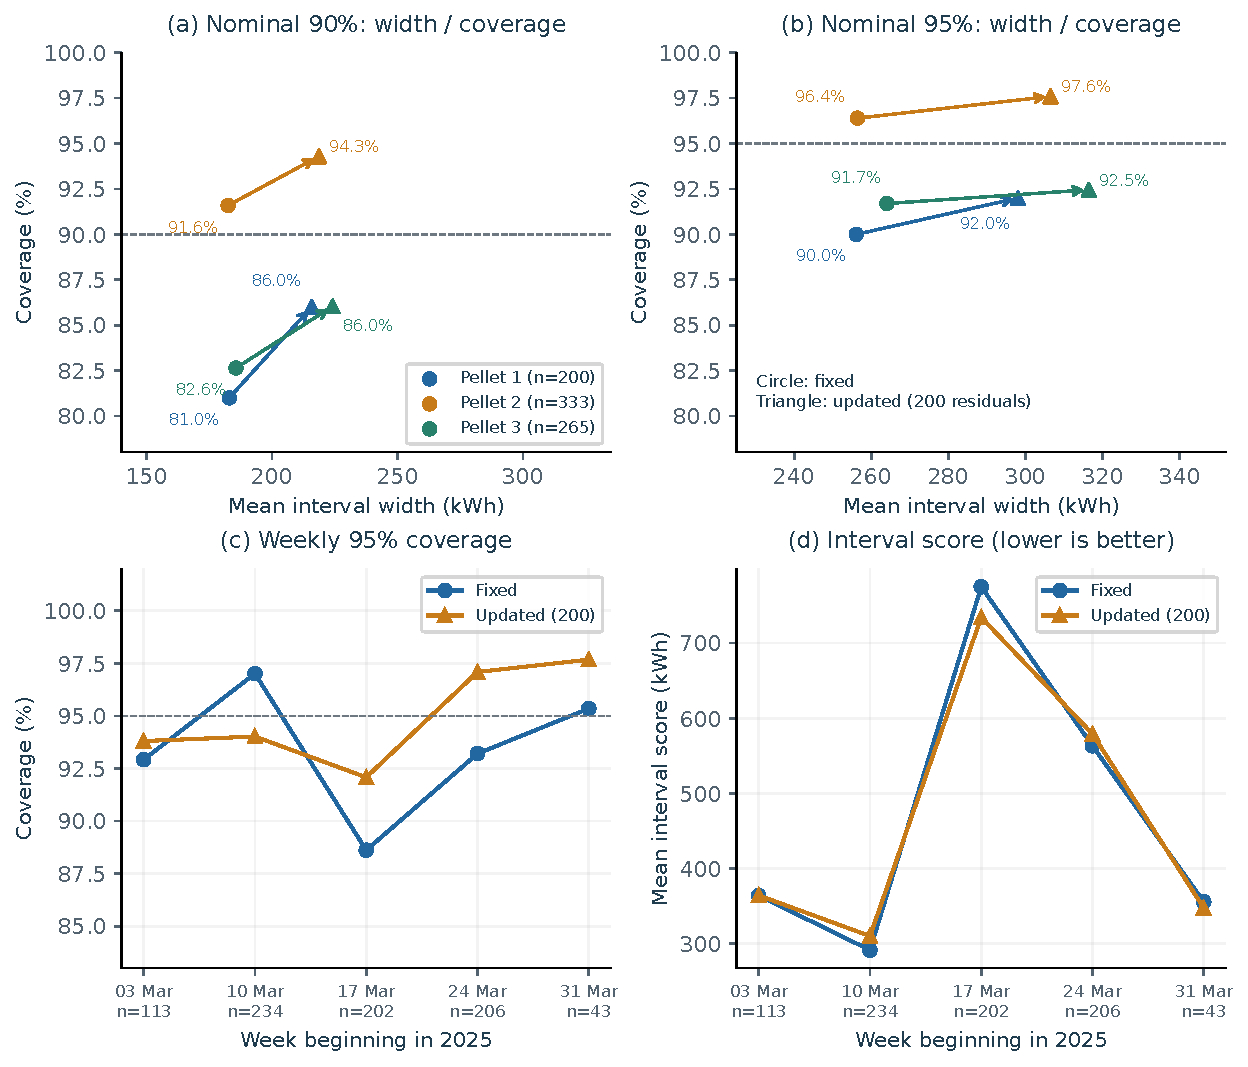
\includegraphics[width=\linewidth]{figures/06_uncertainty_tradeoff.pdf}
\caption{Coverage, width and interval score for the fixed calibration and the exploratory rolling update. (a,b) Line-specific coverage against mean interval width at nominal 90\% and 95\%; arrows connect fixed intervals (circles) to updated intervals (triangles). (c,d) Weekly 95\% coverage and interval score, with sample sizes and partial weeks at the edges; dashed lines mark nominal coverage, and a lower interval score is better. Both policies use the same 798 fixed point predictions.}\label{fig:s_unc}\end{figure}
\FloatBarrier

\section{Matched temporal benchmark}\label{sec:temporal}
The benchmark asks whether the 16 most recent completed same-line operations add information beyond the current-record covariates. Contexts are built within each outer validation week and its training block, a donor must have completed before the target origin (completion is a proxy for data publication), and ties are broken by source row. Requiring 16 donors retains 584 of the 800 development targets. Table~\ref{tab:s_folds} lists the outer and inner sample sizes per week: the inner validation week immediately precedes the outer week and is used only to select the number of epochs of each seed (maximum 40, patience 8); each seed is then refitted from scratch on the complete outer training block and the reported prediction is the mean of the three clipped seed predictions. TFT uses hidden size 32, four attention heads and dropout 0.1; N-HiTS uses three stacks of one block each with two 64-unit layers, pooling kernels 2, 2 and 1 and no frequency downsampling. Both optimize the standardized-target MSE with Adam (learning rate $10^{-3}$, weight decay $10^{-4}$, batch size 64, gradient clipping at 1). The Ridge controls use penalty 10 with current covariates only or with the flattened 16-record window appended. Foundation models run zero-shot with frozen weights: TimesFM~2.5 (\texttt{google/timesfm-2.5-200m-pytorch}, revision \texttt{1d952420}) alone and with its XReg adapter (ridge 10, one call per origin so that no query pools labels from another query's future), and Chronos-2 (\texttt{amazon/chronos-2}, revision \texttt{29ec3766}) with energy only and with its native past/future covariates, cross-query learning disabled, median forecast.

\begin{table}[!htbp]\centering\small
\caption{Sample sizes of the matched temporal benchmark for each outer validation week (week starting on the date shown): outer training records, inner training and inner validation records used for epoch selection, and outer validation targets.}\label{tab:s_folds}
\begin{tabular}{@{}lrrrr@{}}\toprule
Validation week & Outer training & Inner training & Inner validation & Targets \\\midrule
2025-01-25 & 650 & 447 & 141 & 151 \\
2025-02-01 & 869 & 650 & 151 & 133 \\
2025-02-08 & 1066 & 869 & 133 & 151 \\
2025-02-15 & 1279 & 1066 & 151 & 149 \\
\bottomrule
\end{tabular}
\end{table}

\begin{table}[!htbp]\centering\scriptsize
\caption{Matched temporal benchmark by outer validation week (584 targets in total). MAE, RMSE and bias in kWh per record; the last column counts raw predictions below zero before clipping.}\label{tab:s_by_fold}
\begin{tabular}{@{}llrrrrrr@{}}\toprule
Method & Week & $n$ & MAE & RMSE & Bias & WAPE (\%) & Neg. \\\midrule
Ridge, current inputs & 2025-01-25 & 151 & 52.30 & 76.40 & $-11.79$ & 19.54 & 0 \\
Ridge, current inputs & 2025-02-01 & 133 & 63.80 & 90.73 & $-7.07$ & 23.01 & 0 \\
Ridge, current inputs & 2025-02-08 & 151 & 49.89 & 65.99 & $-9.12$ & 19.04 & 0 \\
Ridge, current inputs & 2025-02-15 & 149 & 49.36 & 74.64 & 8.99 & 20.05 & 0 \\
Ridge, full 16-record window & 2025-01-25 & 151 & 67.20 & 85.32 & $-8.06$ & 25.11 & 0 \\
Ridge, full 16-record window & 2025-02-01 & 133 & 74.56 & 99.17 & 3.89 & 26.89 & 1 \\
Ridge, full 16-record window & 2025-02-08 & 151 & 57.26 & 72.77 & $-8.64$ & 21.85 & 1 \\
Ridge, full 16-record window & 2025-02-15 & 149 & 57.96 & 86.21 & 7.89 & 23.55 & 0 \\
TFT & 2025-01-25 & 151 & 52.28 & 79.77 & $-23.90$ & 19.53 & 0 \\
TFT & 2025-02-01 & 133 & 62.73 & 93.12 & $-8.50$ & 22.62 & 0 \\
TFT & 2025-02-08 & 151 & 50.59 & 67.02 & $-15.51$ & 19.31 & 0 \\
TFT & 2025-02-15 & 149 & 50.04 & 76.06 & 3.52 & 20.33 & 0 \\
N-HiTS & 2025-01-25 & 151 & 75.99 & 104.45 & $-22.10$ & 28.39 & 1 \\
N-HiTS & 2025-02-01 & 133 & 73.23 & 105.89 & 7.23 & 26.41 & 0 \\
N-HiTS & 2025-02-08 & 151 & 55.86 & 71.81 & $-0.14$ & 21.32 & 0 \\
N-HiTS & 2025-02-15 & 149 & 56.88 & 85.37 & 4.13 & 23.11 & 0 \\
Chronos-2 + covariates & 2025-01-25 & 151 & 93.58 & 132.60 & $-9.89$ & 34.97 & 0 \\
Chronos-2 + covariates & 2025-02-01 & 133 & 95.82 & 134.05 & $-17.07$ & 34.55 & 0 \\
Chronos-2 + covariates & 2025-02-08 & 151 & 76.22 & 107.60 & $-5.14$ & 29.09 & 0 \\
Chronos-2 + covariates & 2025-02-15 & 149 & 77.61 & 107.81 & $-1.32$ & 31.53 & 0 \\
TimesFM 2.5, energy only & 2025-01-25 & 151 & 106.47 & 143.48 & $-4.31$ & 39.78 & 0 \\
TimesFM 2.5, energy only & 2025-02-01 & 133 & 99.91 & 139.87 & $-17.75$ & 36.03 & 0 \\
TimesFM 2.5, energy only & 2025-02-08 & 151 & 86.53 & 117.84 & $-13.66$ & 33.02 & 0 \\
TimesFM 2.5, energy only & 2025-02-15 & 149 & 93.05 & 120.75 & $-2.09$ & 37.80 & 0 \\
Chronos-2, energy only & 2025-01-25 & 151 & 110.41 & 149.51 & $-11.69$ & 41.25 & 0 \\
Chronos-2, energy only & 2025-02-01 & 133 & 106.11 & 146.84 & $-14.29$ & 38.27 & 0 \\
Chronos-2, energy only & 2025-02-08 & 151 & 91.41 & 124.92 & $-14.48$ & 34.88 & 0 \\
Chronos-2, energy only & 2025-02-15 & 149 & 92.79 & 123.63 & $-6.20$ & 37.70 & 0 \\
TimesFM 2.5 + XReg & 2025-01-25 & 151 & 235.92 & 1256.28 & 143.41 & 88.15 & 0 \\
TimesFM 2.5 + XReg & 2025-02-01 & 133 & 81.20 & 119.73 & $-26.73$ & 29.28 & 0 \\
TimesFM 2.5 + XReg & 2025-02-08 & 151 & 59.70 & 83.81 & $-10.57$ & 22.78 & 0 \\
TimesFM 2.5 + XReg & 2025-02-15 & 149 & 67.39 & 96.30 & $-0.91$ & 27.38 & 0 \\
\bottomrule
\end{tabular}
\end{table}

\begin{table}[!htbp]\centering\scriptsize
\caption{Matched temporal benchmark by pelleting line (149, 257 and 178 targets on Pellet~1, 2 and 3).}\label{tab:s_by_line}
\begin{tabular}{@{}llrrrrrr@{}}\toprule
Method & Line & $n$ & MAE & RMSE & Bias & WAPE (\%) & Neg. \\\midrule
Ridge, current inputs & Pellet 1 & 149 & 48.96 & 78.25 & $-1.80$ & 22.11 & 0 \\
Ridge, current inputs & Pellet 2 & 257 & 48.13 & 65.50 & $-17.04$ & 19.29 & 0 \\
Ridge, current inputs & Pellet 3 & 178 & 65.20 & 90.22 & 10.62 & 20.57 & 0 \\
Ridge, full 16-record window & Pellet 1 & 149 & 58.89 & 81.23 & $-4.82$ & 26.60 & 0 \\
Ridge, full 16-record window & Pellet 2 & 257 & 57.71 & 74.63 & $-13.50$ & 23.13 & 2 \\
Ridge, full 16-record window & Pellet 3 & 178 & 77.19 & 103.31 & 18.87 & 24.35 & 0 \\
TFT & Pellet 1 & 149 & 49.21 & 79.60 & $-6.38$ & 22.22 & 0 \\
TFT & Pellet 2 & 257 & 47.22 & 66.22 & $-19.56$ & 18.93 & 0 \\
TFT & Pellet 3 & 178 & 66.65 & 94.32 & $-3.26$ & 21.03 & 0 \\
N-HiTS & Pellet 1 & 149 & 62.07 & 92.71 & $-10.29$ & 28.03 & 0 \\
N-HiTS & Pellet 2 & 257 & 56.85 & 76.30 & $-11.49$ & 22.78 & 1 \\
N-HiTS & Pellet 3 & 178 & 80.14 & 111.84 & 15.20 & 25.28 & 0 \\
Chronos-2 + covariates & Pellet 1 & 149 & 81.78 & 115.21 & $-11.52$ & 36.93 & 0 \\
Chronos-2 + covariates & Pellet 2 & 257 & 70.10 & 98.97 & $-8.20$ & 28.09 & 0 \\
Chronos-2 + covariates & Pellet 3 & 178 & 110.94 & 150.47 & $-5.12$ & 35.00 & 0 \\
TimesFM 2.5, energy only & Pellet 1 & 149 & 97.50 & 132.42 & $-13.96$ & 44.04 & 0 \\
TimesFM 2.5, energy only & Pellet 2 & 257 & 78.83 & 107.38 & $-4.76$ & 31.59 & 0 \\
TimesFM 2.5, energy only & Pellet 3 & 178 & 120.84 & 157.29 & $-11.70$ & 38.12 & 0 \\
Chronos-2, energy only & Pellet 1 & 149 & 99.07 & 134.29 & $-16.12$ & 44.75 & 0 \\
Chronos-2, energy only & Pellet 2 & 257 & 81.34 & 111.66 & $-8.05$ & 32.60 & 0 \\
Chronos-2, energy only & Pellet 3 & 178 & 127.79 & 167.34 & $-12.96$ & 40.31 & 0 \\
TimesFM 2.5 + XReg & Pellet 1 & 149 & 65.78 & 101.22 & $-13.49$ & 29.71 & 0 \\
TimesFM 2.5 + XReg & Pellet 2 & 257 & 61.86 & 87.28 & $-9.45$ & 24.79 & 0 \\
TimesFM 2.5 + XReg & Pellet 3 & 178 & 223.48 & 1159.18 & 116.90 & 70.50 & 0 \\
\bottomrule
\end{tabular}
\end{table}

\begin{table}[!htbp]\centering\small
\caption{Individual seeds of the locally trained temporal models on the 584 matched targets. The reported ensemble averages the three clipped predictions, so its MAE is not the mean of the three seed MAEs.}\label{tab:s_seeds}
\begin{tabular}{@{}lrrrrrr@{}}\toprule
Method & Seed & $n$ & MAE & RMSE & Bias & WAPE (\%) \\\midrule
N-HiTS & 11 & 584 & 71.91 & 97.92 & $-19.03$ & 27.35 \\
N-HiTS & 29 & 584 & 70.76 & 98.09 & 11.49 & 26.91 \\
N-HiTS & 47 & 584 & 69.39 & 97.15 & $-1.61$ & 26.39 \\
TFT & 11 & 584 & 55.31 & 79.72 & $-12.47$ & 21.04 \\
TFT & 29 & 584 & 58.17 & 84.25 & $-7.78$ & 22.13 \\
TFT & 47 & 584 & 56.43 & 82.42 & $-13.44$ & 21.46 \\
\bottomrule
\end{tabular}
\end{table}

\begin{table}[!htbp]\centering\footnotesize
\caption{Paired MAE differences relative to current-input Ridge on the 584 matched targets (positive values would favour the alternative): marginal 95\% and family-adjusted 99.29\% block-bootstrap intervals for the seven contrasts (5,000 replicates, blocks of three observed origin dates, seed 20260922), and the 95\% interval of each method's own MAE.}\label{tab:s_paired}
\begin{tabular}{@{}lrlll@{}}\toprule
Method & Improvement (kWh) & 95\% interval & 99.29\% interval & MAE 95\% interval \\\midrule
Ridge, current inputs & 0.000 & [0.000, 0.000] & [0.000, 0.000] & [48.77, 59.01] \\
Ridge, full 16-record window & $-10.403$ & [$-13.435$, $-7.635$] & [$-14.518$, $-6.804$] & [57.37, 70.88] \\
TFT & $-0.105$ & [$-2.199$, 2.318] & [$-2.914$, 3.325] & [49.50, 58.55] \\
N-HiTS & $-11.733$ & [$-19.077$, $-6.789$] & [$-21.922$, $-5.809$] & [57.76, 74.67] \\
Chronos-2 + covariates & $-31.981$ & [$-38.087$, $-27.675$] & [$-41.104$, $-26.922$] & [79.03, 93.31] \\
TimesFM 2.5, energy only & $-42.852$ & [$-50.175$, $-36.525$] & [$-53.336$, $-35.112$] & [90.10, 104.11] \\
Chronos-2, energy only & $-46.477$ & [$-54.303$, $-40.813$] & [$-57.634$, $-39.515$] & [93.14, 108.92] \\
TimesFM 2.5 + XReg & $-58.576$ & [$-152.154$, $-14.414$] & [$-203.361$, $-11.970$] & [67.58, 205.10] \\
\bottomrule
\end{tabular}
\end{table}


The three extreme TimesFM XReg predictions of the first validation week (about 2,753, 9,239 and 12,203~kWh for observed values of 185.4, 142.4 and 70.9~kWh on Pellet~3) arise from contexts in which the dosed mass of the 16 donors was almost constant, so the standardized current mass lay roughly 1,100--1,467 historical standard deviations from the local mean; an independent float64 reconstruction of the adapter reproduced the extrapolation. They account for the first-week MAE of 235.9~kWh and RMSE of 1,256.3~kWh of that variant in Table~\ref{tab:s_by_fold} and are retained in every reported metric. Figures~\ref{fig:s_strata} and \ref{fig:s_all} show the stratified MAE and all 4,672 predictions.

\begin{figure}[!htbp]\centering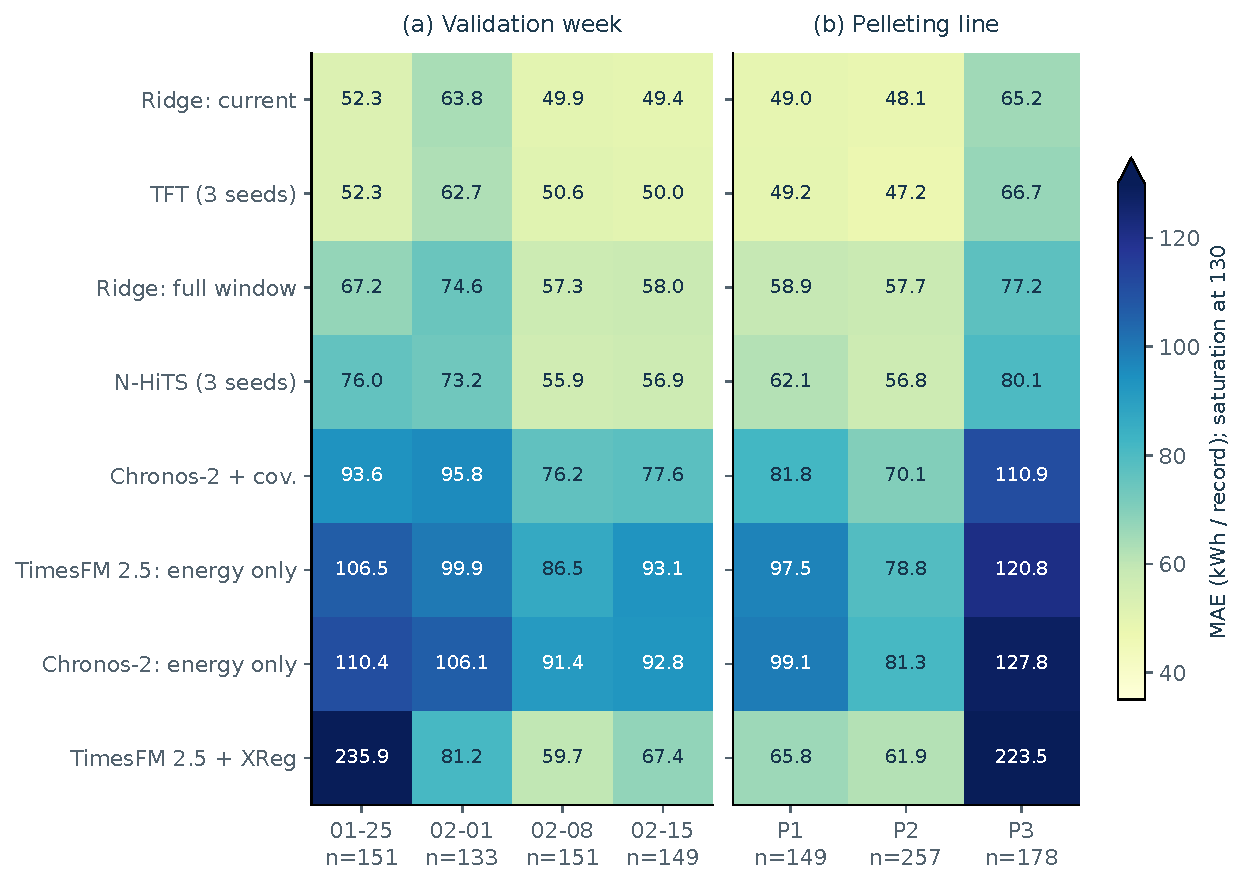
\includegraphics[width=\linewidth]{figures/09_gpu_stratification.pdf}
\caption{MAE by pelleting line and by validation week for the eight methods of the matched benchmark, in kWh per record; labels give the number of targets in each stratum. The colour scale ends at 130~kWh so that differences among the lower errors remain readable, while printed values preserve every result above that limit.}\label{fig:s_strata}\end{figure}

\begin{figure}[!htbp]\centering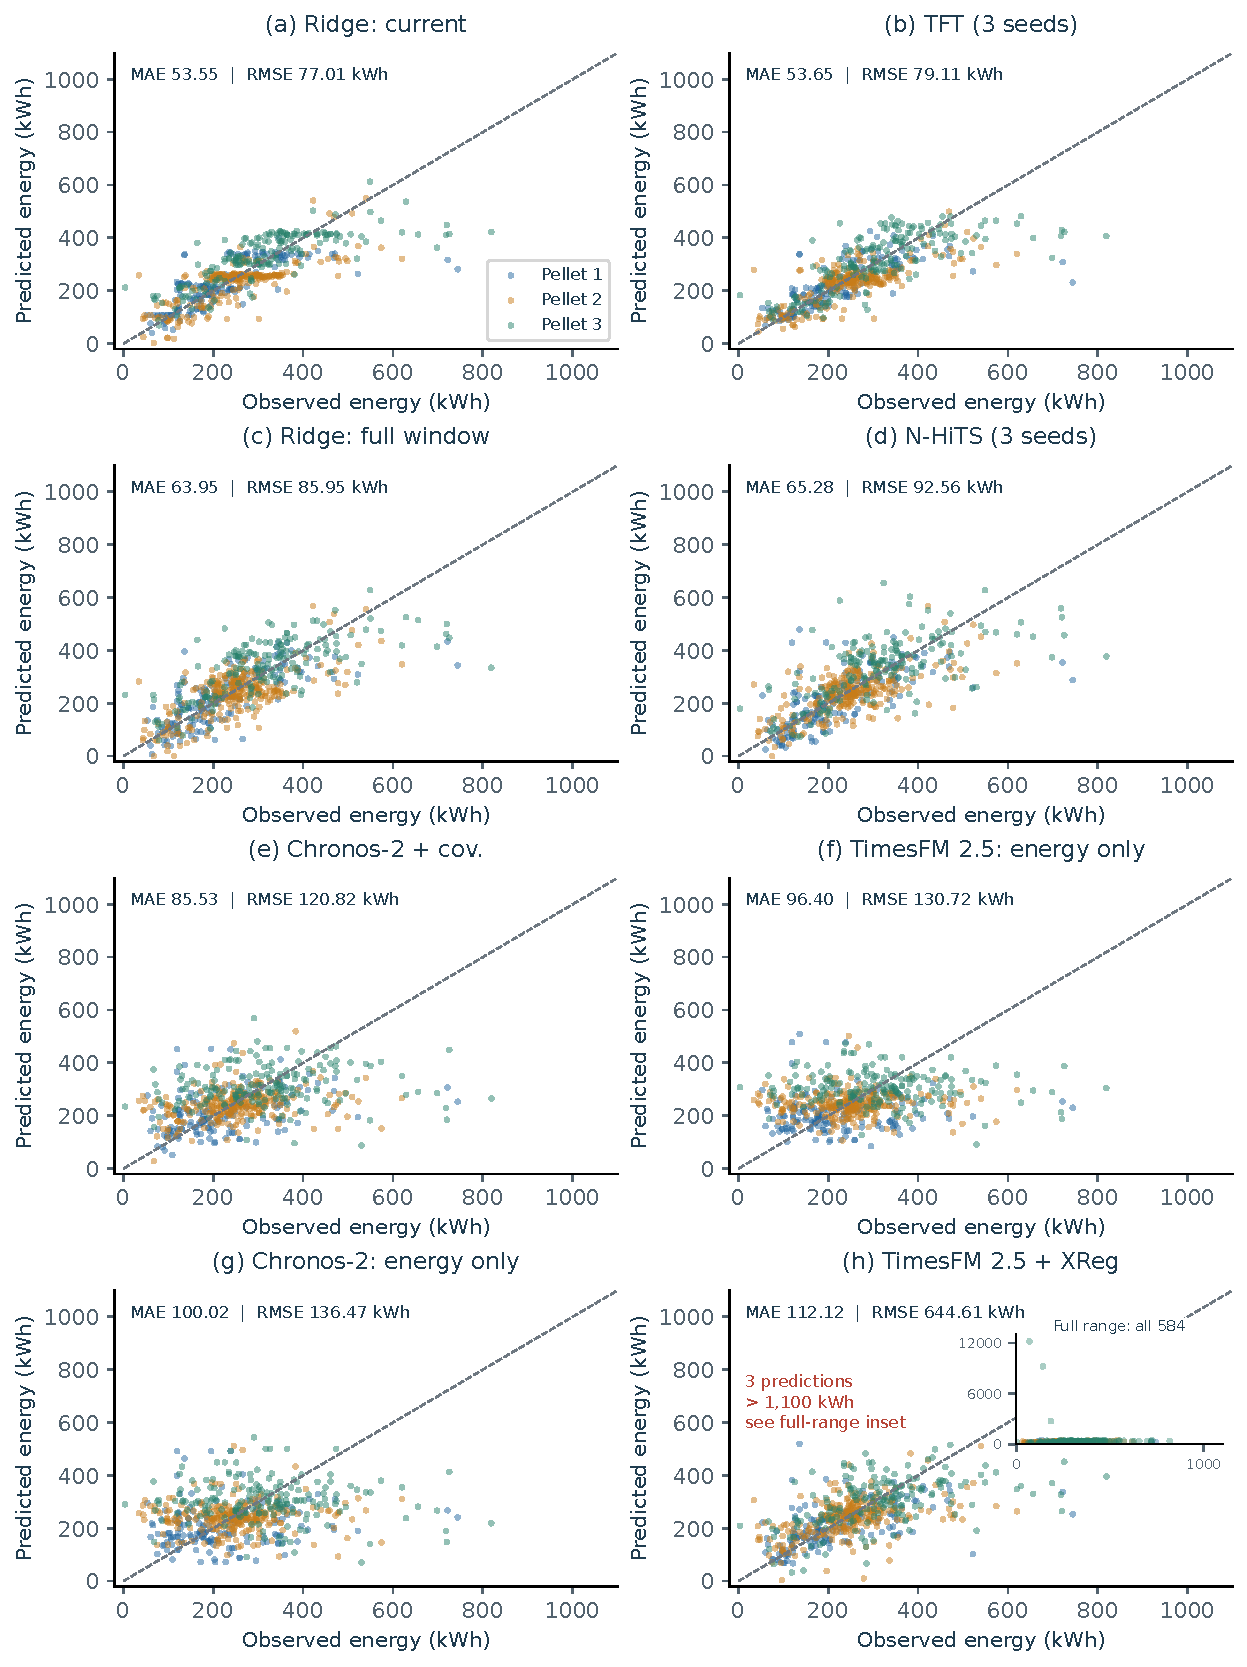
\includegraphics[width=.9\linewidth]{figures/10_gpu_all_predictions.pdf}
\caption{All 4,672 predictions of the matched comparison: eight methods on 584 identical records. Colours identify the three lines and the dashed diagonal marks equality. The main axes share a 0--1,100~kWh range; the TimesFM XReg panel adds a full-range inset containing its three extreme predictions. MAE and RMSE use the complete data in every panel.}\label{fig:s_all}\end{figure}
\FloatBarrier

\section{Computational diagnostics}\label{sec:compute}
The GPU run repeated the frozen protocol on an NVIDIA RTX PRO 5000 Blackwell (48~GB) in float32 with TF32 disabled: 24 supervised refits (two architectures $\times$ four weeks $\times$ three seeds) in 532~s of wall time and 16 foundation-model fold variants in 282~s, with a peak of 915~MiB of CUDA memory; Ridge and the JAX XReg solver ran on CPU. Table~\ref{tab:s_cpu_gpu} compares the CPU and GPU runs, Table~\ref{tab:s_epochs} the epochs selected on each device and Table~\ref{tab:s_numdiff} the per-method prediction differences. Within the GPU run, the 24 saved checkpoints were reloaded and their inference at batch size 8 compared with the stored batch-64 inference, together with four Chronos covariate batch-size checks: all 28 checks passed with a maximum difference of $7.63\times10^{-5}$~kWh. Fresh CPU and GPU fits of the same seed can follow different optimization trajectories, which explains the TFT and N-HiTS differences; the frozen TimesFM variants and univariate Chronos agree across devices to below $2\times10^{-4}$~kWh, whereas Chronos-2 with covariates differs by up to 57.04~kWh on individual records (median 0.86~kWh).

To trace the latter, the installed Chronos preprocessing and instance normalization were applied on both devices to the 584 contexts, giving 6,424 target/covariate channels. Among the 1,097 channels whose history is constant in float32, 694 showed normalized-context differences above 0.1, with a maximum of 0.8814 in the transformed (inverse-hyperbolic-sine) coordinates; no non-constant channel exceeded the threshold. The implementation substitutes a small scale only when the computed scale is exactly zero, so round-off variances of constant channels can be amplified differently by the two devices' reductions. This is a mechanism consistent with the observed prediction differences, not an end-to-end attribution of every residual, and the primary predictions were not modified.

\begin{table}[!htbp]\centering\footnotesize
\caption{CPU and GPU runs of the same protocol on the 584 matched targets. TFT and N-HiTS were trained afresh on each device; foundation-model weights were frozen on both.}\label{tab:s_cpu_gpu}
\begin{tabular}{@{}lrrrrr@{}}\toprule
Method & CPU MAE & GPU MAE & CPU RMSE & GPU RMSE & GPU $-$ CPU MAE \\\midrule
Ridge, current inputs & 53.5457 & 53.5457 & 77.0140 & 77.0140 & 0.0000 \\
Ridge, full 16-record window & 63.9491 & 63.9491 & 85.9487 & 85.9487 & 0.0000 \\
TFT & 53.2484 & 53.6507 & 79.0792 & 79.1050 & 0.4023 \\
N-HiTS & 66.3527 & 65.2784 & 93.6651 & 92.5581 & $-1.0744$ \\
Chronos-2 + covariates & 85.6480 & 85.5268 & 121.1050 & 120.8235 & $-0.1211$ \\
TimesFM 2.5, energy only & 96.3980 & 96.3980 & 130.7237 & 130.7237 & $-0.0000$ \\
Chronos-2, energy only & 100.0225 & 100.0225 & 136.4695 & 136.4695 & $-0.0000$ \\
TimesFM 2.5 + XReg & 112.1213 & 112.1213 & 644.6068 & 644.6068 & $-0.0000$ \\
\bottomrule
\end{tabular}
\end{table}

\begin{table}[!htbp]\centering\footnotesize
\caption{Epoch selected on the inner validation week for every model, outer week and seed, on CPU and on GPU (maximum 40 epochs, patience 8).}\label{tab:s_epochs}
\begin{tabular}{@{}llrrr@{}}\toprule
Model & Week & Seed & CPU epoch & GPU epoch \\\midrule
TFT & 2025-01-25 & 11 & 3 & 3 \\
TFT & 2025-01-25 & 29 & 24 & 14 \\
TFT & 2025-01-25 & 47 & 9 & 9 \\
N-HiTS & 2025-01-25 & 11 & 11 & 11 \\
N-HiTS & 2025-01-25 & 29 & 9 & 9 \\
N-HiTS & 2025-01-25 & 47 & 10 & 10 \\
TFT & 2025-02-01 & 11 & 2 & 2 \\
TFT & 2025-02-01 & 29 & 4 & 5 \\
TFT & 2025-02-01 & 47 & 2 & 2 \\
N-HiTS & 2025-02-01 & 11 & 12 & 12 \\
N-HiTS & 2025-02-01 & 29 & 9 & 9 \\
N-HiTS & 2025-02-01 & 47 & 22 & 30 \\
TFT & 2025-02-08 & 11 & 7 & 1 \\
TFT & 2025-02-08 & 29 & 6 & 8 \\
TFT & 2025-02-08 & 47 & 3 & 3 \\
N-HiTS & 2025-02-08 & 11 & 15 & 15 \\
N-HiTS & 2025-02-08 & 29 & 8 & 8 \\
N-HiTS & 2025-02-08 & 47 & 19 & 19 \\
TFT & 2025-02-15 & 11 & 7 & 7 \\
TFT & 2025-02-15 & 29 & 2 & 6 \\
TFT & 2025-02-15 & 47 & 5 & 14 \\
N-HiTS & 2025-02-15 & 11 & 11 & 6 \\
N-HiTS & 2025-02-15 & 29 & 9 & 9 \\
N-HiTS & 2025-02-15 & 47 & 13 & 13 \\
\bottomrule
\end{tabular}
\end{table}

\begin{table}[!htbp]\centering\small
\caption{Absolute CPU--GPU prediction differences per method over the 584 matched targets (kWh).}\label{tab:s_numdiff}
\begin{tabular}{@{}lrrr@{}}\toprule
Method & Mean & Maximum & Median \\\midrule
Ridge, current inputs & 0.000000 & 0.000000 & 0.000000 \\
Ridge, full 16-record window & 0.000000 & 0.000000 & 0.000000 \\
TFT & 9.431759 & 56.837992 & 8.269961 \\
N-HiTS & 9.881184 & 47.780848 & 6.692332 \\
Chronos-2 + covariates & 2.386194 & 57.041779 & 0.859741 \\
TimesFM 2.5, energy only & 0.000014 & 0.000092 & 0.000000 \\
Chronos-2, energy only & 0.000015 & 0.000183 & 0.000000 \\
TimesFM 2.5 + XReg & 0.000007 & 0.000061 & 0.000000 \\
\bottomrule
\end{tabular}
\end{table}


\begin{table}[!htbp]\centering\small
\caption{Software environment of the archived runs and pretrained checkpoints.}\label{tab:s_versions}
\begin{tabular}{@{}ll@{}}\toprule
Component & Version / revision \\\midrule
Python & 3.13.13 \\
PyTorch & 2.14.0+cu130 (CUDA 13.0) \\
NeuralForecast & 3.2.2 \\
timesfm & 3.0.2 \\
chronos-forecasting & 2.3.2 \\
NumPy / pandas / scikit-learn & 2.5.1 / 2.3.3 / 1.9.0 \\
TimesFM 2.5 checkpoint & \texttt{google/timesfm-2.5-200m-pytorch} \\
\quad revision & \texttt{1d952420fba87f3c6dee4f240de0f1a0fbc790e3} \\
Chronos-2 checkpoint & \texttt{amazon/chronos-2} \\
\quad revision & \texttt{29ec3766d36d6f73f0696f85560a422f50e8498c} \\\bottomrule
\end{tabular}
\end{table}
\FloatBarrier

\section{Reproducibility and data access}\label{sec:repro}
The public repository \url{https://github.com/fmarrabal/pelleting-energy-baseline-real-data} (release \texttt{v4-submission}) contains the original scientific scripts, the figure scripts, the aggregate result tables used to build this document, the frozen model configuration and the LaTeX sources of the manuscript and of this supplement. Its \texttt{reproduce.py} entry point verifies the file inventory against SHA-256 manifests, recompiles the manuscript and, once the record-level tables are in place, recomputes the metrics and regenerates every figure. Frozen artefacts are identified by fingerprint: the cleaned analytical table (\texttt{c462f92a\ldots}), the frozen calibrated model (\texttt{b355bf28\ldots}), the evaluation protocol (\texttt{919a53ec\ldots}) and the source workbook (\texttt{d5968030\ldots}).

The industrial production and electricity records, the cleaned analytical table and every record-level table derived from them (per-record predictions, residuals, intervals and contexts) belong to the plant and are not distributed publicly. They are available from the corresponding author (\href{mailto:fmarrabal@ual.es}{fmarrabal@ual.es}) on reasonable request, subject to the data owner's agreement; the repository's manifests allow a recipient to verify that the received files are the ones used in the study.
\end{document}
